\documentclass[border=8pt]{standalone}
\usepackage[T1]{fontenc}
\usepackage{tikz}
\usepackage{amsmath,amssymb}
\usetikzlibrary{arrows.meta,positioning,shapes.geometric,fit,calc,backgrounds}

\definecolor{promptblue}{HTML}{DAEAF6}
\definecolor{promptborder}{HTML}{5B9BD5}
\definecolor{featureblue}{HTML}{4472C4}
\definecolor{filtergray}{HTML}{E2EFDA}
\definecolor{filterborder}{HTML}{A9D18E}
\definecolor{registrybg}{HTML}{FFF2CC}
\definecolor{registryborder}{HTML}{BF9000}
\definecolor{corralgreen}{HTML}{70AD47}
\definecolor{expertorg}{HTML}{ED7D31}
\definecolor{expertyellow}{HTML}{FFF2CC}
\definecolor{ucbblue}{HTML}{D6E4F0}
\definecolor{ucbborder}{HTML}{2F5496}
\definecolor{rewardpink}{HTML}{F4CCCC}
\definecolor{rewardborder}{HTML}{CC4125}
\definecolor{storegray}{HTML}{D9D9D9}
\definecolor{feedbackred}{HTML}{CC4125}
\definecolor{formulacolor}{HTML}{BF6900}
\definecolor{modelhl}{HTML}{BDD7EE}

\begin{document}
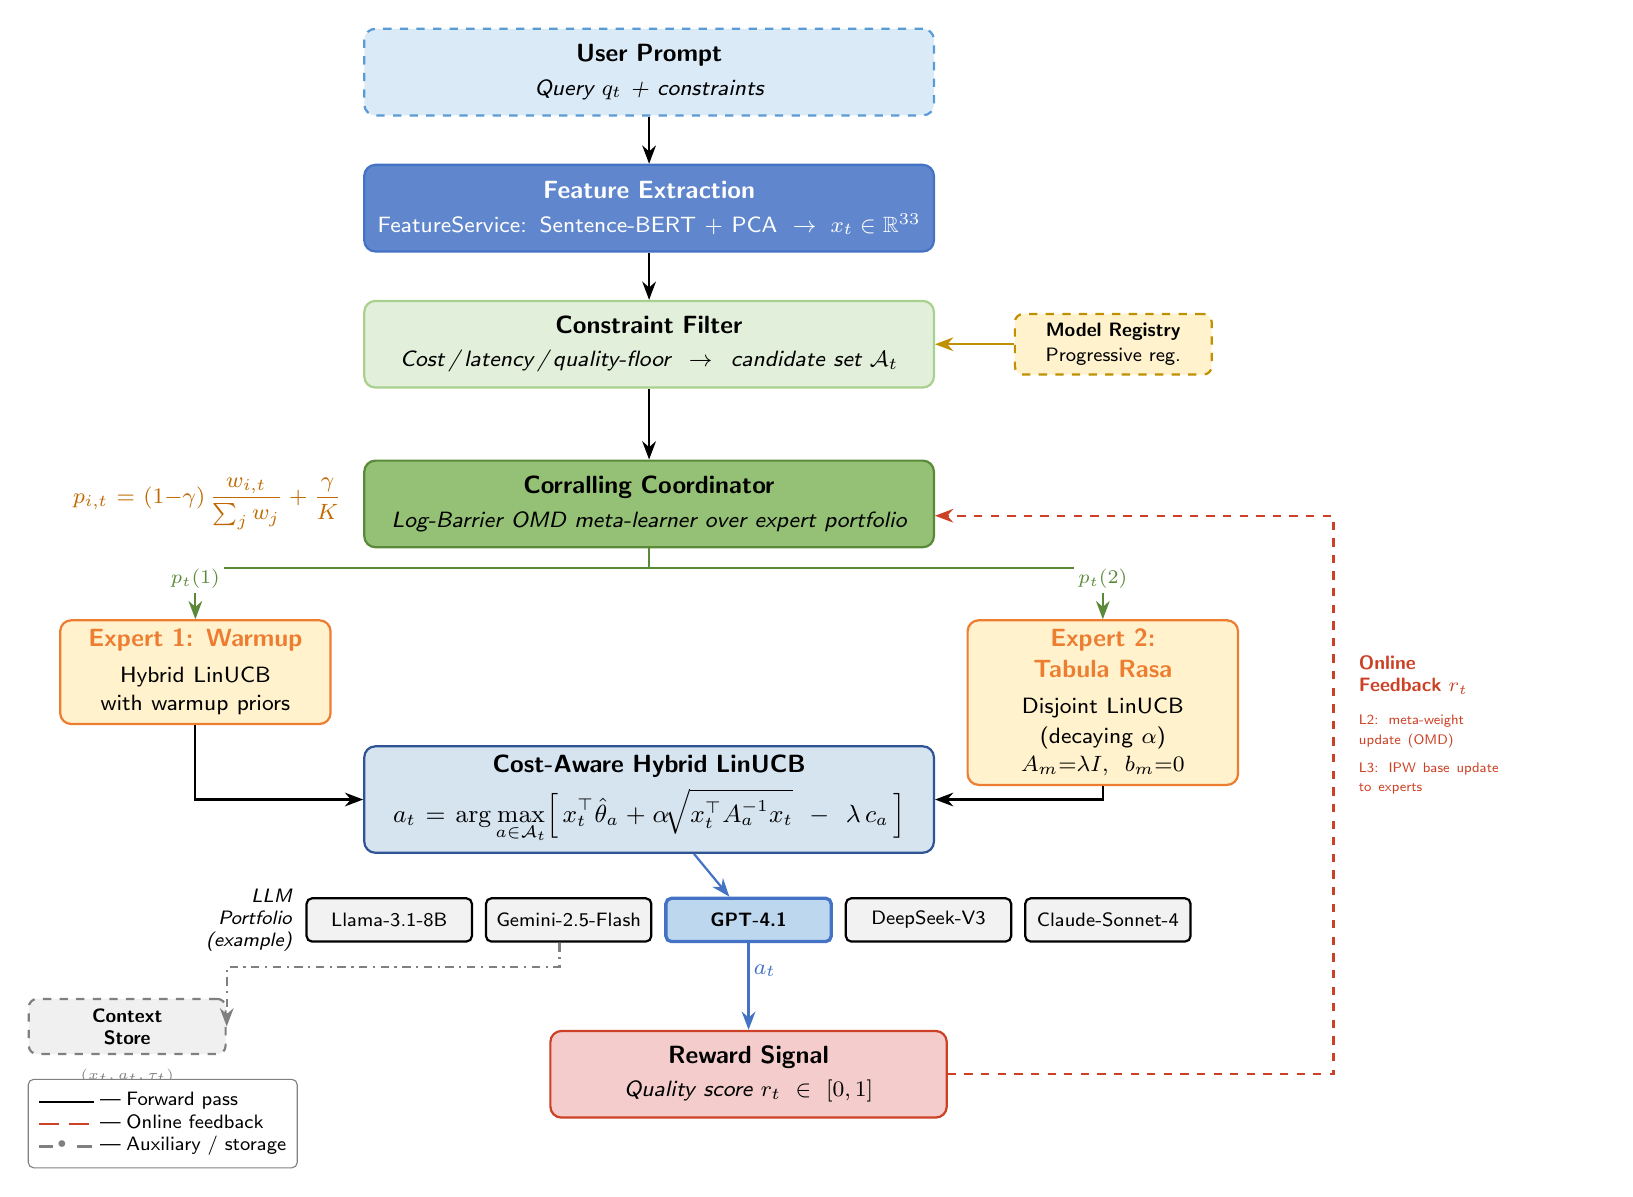
\begin{tikzpicture}[
    >=Stealth,
    node distance=0.6cm,
    every node/.style={font=\sffamily\small},
    box/.style={
        rectangle, rounded corners=4pt, draw, thick,
        minimum width=7.2cm, minimum height=1.1cm,
        text width=7cm, align=center,
    },
    smallbox/.style={
        rectangle, rounded corners=3pt, draw, thick,
        minimum width=2.5cm, minimum height=0.7cm,
        align=center,
    },
    modelbox/.style={
        rectangle, rounded corners=2pt, draw, thick,
        minimum width=2.1cm, minimum height=0.55cm,
        align=center, font=\sffamily\scriptsize,
    },
    expertbox/.style={
        rectangle, rounded corners=4pt, draw=expertorg, thick,
        fill=expertyellow, minimum width=3.4cm, minimum height=1.1cm,
        text width=3.2cm, align=center,
    },
    arrowlabel/.style={font=\sffamily\scriptsize, fill=white, inner sep=1.5pt},
    feedbackarrow/.style={->, thick, dashed, feedbackred},
    auxarrow/.style={->, thick, dash dot, gray},
]

% =====================================================================
% NODES
% =====================================================================

% 1. User Prompt
\node[box, draw=promptborder, fill=promptblue, dashed, thick] (prompt)
    {\textbf{User Prompt}\\[1pt]
     {\footnotesize\itshape Query $q_t$ + constraints}};

% 2. Feature Extraction
\node[box, draw=featureblue, fill=featureblue!85!white, text=white,
      below=of prompt] (features)
    {\textbf{Feature Extraction}\\[1pt]
     {\footnotesize FeatureService: Sentence-BERT + PCA
      $\;\to\; x_t \in \mathbb{R}^{33}$}};

% 3. Constraint Filter
\node[box, draw=filterborder, fill=filtergray,
      below=of features] (filter)
    {\textbf{Constraint Filter}\\[1pt]
     {\footnotesize\itshape Cost\,/\,latency\,/\,quality-floor
      $\;\to\;$ candidate set $\mathcal{A}_t$}};

% Model Registry (side)
\node[smallbox, draw=registryborder, fill=registrybg, dashed,
      right=1.0cm of filter, font=\sffamily\scriptsize,
      text width=2.0cm] (registry)
    {\textbf{Model Registry}\\[1pt] Progressive reg.};

% 4. Corralling Coordinator
\node[box, draw=corralgreen!80!black, fill=corralgreen!75!white,
      below=0.9cm of filter] (corral)
    {\textbf{Corralling Coordinator}\\[1pt]
     {\footnotesize\itshape Log-Barrier OMD meta-learner over expert portfolio}};

% Corralling formula (left side)
\node[anchor=east, font=\sffamily\footnotesize, text=formulacolor,
      left=0.15cm of corral.west, text width=3.6cm, align=right] (corraleq)
    {$\displaystyle p_{i,t} = (1{-}\gamma)\,
     \frac{w_{i,t}}{\sum_j w_j} + \frac{\gamma}{K}$};

% 5. Expert branches
\node[expertbox, below left=0.9cm and 0.4cm of corral] (expert1)
    {\textbf{\color{expertorg}Expert 1: Warmup}\\[2pt]
     {\footnotesize Hybrid LinUCB}\\[-1pt]
     {\footnotesize with warmup priors}};

\node[expertbox, below right=0.9cm and 0.4cm of corral] (expert2)
    {\textbf{\color{expertorg}Expert 2: Tabula Rasa}\\[2pt]
     {\footnotesize Disjoint LinUCB (decaying $\alpha$)}\\[-1pt]
     {\footnotesize $A_m{=}\lambda I,\; b_m{=}0$}};

% 6. Cost-Aware UCB (shared selection objective)
\node[box, draw=ucbborder, fill=ucbblue,
      below=1.6cm of corral, yshift=-0.9cm] (ucb)
    {\textbf{Cost-Aware Hybrid LinUCB}\\[3pt]
     $\displaystyle a_t = \arg\max_{a \in \mathcal{A}_t}\!
     \Big[\, x_t^\top \hat{\theta}_a
     + \alpha\!\sqrt{x_t^\top A_a^{-1} x_t}
     \;-\; \lambda\, c_a \,\Big]$};

% 7. LLM Portfolio
\node[below=0.6cm of ucb, font=\sffamily\scriptsize, anchor=north]
    (portlabel) {};

\node[modelbox, fill=gray!10, below=0.55cm of ucb, xshift=-3.3cm]
    (m1) {Llama-3.1-8B};
\node[modelbox, fill=gray!10, right=0.15cm of m1]
    (m2) {Gemini-2.5-Flash};
\node[modelbox, fill=modelhl, right=0.15cm of m2, line width=1.2pt,
      draw=featureblue]
    (m3) {\textbf{GPT-4.1}};
\node[modelbox, fill=gray!10, right=0.15cm of m3]
    (m4) {DeepSeek-V3};
\node[modelbox, fill=gray!10, right=0.15cm of m4]
    (m5) {Claude-Sonnet-4};

% LLM portfolio label
\node[font=\sffamily\scriptsize\itshape, anchor=east,
      text width=1.5cm, align=right,
      left=0.05cm of m1.west] (plabel) {LLM Portfolio\\(example)};

% 8. Context Store
\node[smallbox, draw=gray, fill=storegray!40, dashed,
      below left=0.7cm and 1.0cm of m1.south west,
      font=\sffamily\scriptsize, text width=1.6cm] (store)
    {\textbf{Context}\\[0pt]\textbf{Store}};
\node[font=\sffamily\tiny, below=0.05cm of store, text=gray]
    {$(x_t, a_t, \tau_t)$};

% 9. Reward Signal
\node[box, draw=rewardborder, fill=rewardpink,
      minimum width=5cm, text width=4.8cm,
      below=1.1cm of m3] (reward)
    {\textbf{Reward Signal}\\[1pt]
     {\footnotesize\itshape Quality score $r_t \in [0,1]$}};

% =====================================================================
% FORWARD-PASS ARROWS (solid)
% =====================================================================
\draw[->, thick] (prompt) -- (features);
\draw[->, thick] (features) -- (filter);
\draw[->, thick] (filter) -- (corral);
\draw[->, thick, registryborder] (registry) -- (filter);

% Corral → experts
\draw[->, thick, corralgreen!80!black]
    (corral.south) -- ++(0,-0.25) -| (expert1.north)
    node[arrowlabel, pos=0.75, above] {$p_t(1)$};
\draw[->, thick, corralgreen!80!black]
    (corral.south) -- ++(0,-0.25) -| (expert2.north)
    node[arrowlabel, pos=0.75, above] {$p_t(2)$};

% Experts → UCB
\draw[->, thick] (expert1.south) |- (ucb.west);
\draw[->, thick] (expert2.south) |- (ucb.east);

% UCB → selected model
\draw[->, thick, featureblue] (ucb) -- (m3);

% Selected model → reward
\draw[->, thick, featureblue] (m3.south) -- ++(0,-0.35)
    node[arrowlabel, right, font=\sffamily\footnotesize,
         text=featureblue] {$a_t$}
    -- (reward.north);

% =====================================================================
% FEEDBACK ARROWS (dashed red)
% =====================================================================
% Reward → corral + experts (right side)
\coordinate (fbright) at ([xshift=1.8cm]m5.east);

\draw[feedbackarrow] (reward.east) -| (fbright)
    |- ([yshift=-0.15cm]corral.east);

% Feedback labels
\node[anchor=west, font=\sffamily\scriptsize, text=feedbackred,
      text width=3.0cm, align=left]
    at ([xshift=0.2cm]fbright |- expert1.south)
    {\textbf{Online}\\[0pt]\textbf{Feedback} $r_t$\\[4pt]
     {\tiny L2: meta-weight}\\[-1pt]
     {\tiny update (OMD)}\\[2pt]
     {\tiny L3: IPW base update}\\[-1pt]
     {\tiny to experts}};

% =====================================================================
% AUXILIARY (dash-dot gray): Context Store
% =====================================================================
\draw[auxarrow] ([xshift=-2.4cm]m3.south) -- ++(0,-0.3) -| (store.east);

% =====================================================================
% LEGEND
% =====================================================================
\node[anchor=north west, draw=gray, rounded corners=2pt,
      fill=white, inner sep=4pt,
      font=\sffamily\scriptsize]
    at ([yshift=-0.3cm]store.south west) (legend) {
    \begin{tabular}{@{}l@{\;—\;}l@{}}
    \rule[0.3ex]{0.7cm}{1pt}                          & Forward pass \\
    {\color{feedbackred}\rule[0.3ex]{0.25cm}{1pt}\,
     \rule[0.3ex]{0.25cm}{1pt}}                        & Online feedback \\
    {\color{gray}\rule[0.3ex]{0.18cm}{1pt}\,\raisebox{0.3ex}{\tiny$\bullet$}\,
     \rule[0.3ex]{0.18cm}{1pt}}                        & Auxiliary / storage \\
    \end{tabular}
};

\end{tikzpicture}
\end{document}
